\chapter{Revisão de Literatura (ou Referencial Teórico).}

O que já tem escrito no tema que você escolheu?

\section{Primeira seção da Revisão}

Para incluir uma referência em seu trabalho, como por exemplo \cite{Autor1}, use o comando \verb!\cite{<rótulo>}!, 
onde \verb!<rótulo>! indica uma referência que você criou no arquivo \verb!referencias.bib! (que está na pasta \verb!pos-textual/referencias!). 
Um outro exemplo de referência com mais de três autores \cite{Autor3}.

Se você quiser fazer uma citação com mais de três linhas, use o ambiente \verb!citacao!. Veja um exemplo abaixo.

\begin{citacao}
A citação com mais de três linhas tem fonte com tamanho 10 pt, espaço simples entre 
linhas e recuo de 4 cm da margem esquerda. A citação com mais de três linhas tem fonte 
com tamanho 10 pt, espaço simples entre linhas e recuo de 4 cm da margem esquerda. 
A citação com mais de três linhas tem fonte com tamanho 10 pt, espaço simples entre 
linhas e recuo de 4 cm da margem esquerda. A citação com mais de três linhas tem fonte 
com tamanho 10 pt, espaço simples entre linhas e recuo de 4 cm da margem esquerda \cite[p. 11]{Autor2}. 
(Observação: para indicar a página na referência, como ``p. 11'' nesse exemplo, use o 
comando \verb!\cite[p. 11]{<rótulo>}!.)
\end{citacao}

A Tabela~\ref{tabelateste1} é um exemplo de como ficará uma tabela no seu texto. Note que a 
legenda fica na parte superior e tem fonte com tamanho 10 pt (além de espaço simples entre linhas, como 
você pode notar na Tabela~\ref{tabelateste2}).

\begin{table}[htb]
 \centering
 \caption{Exemplo de tabela.}
 \begin{tabular}{|c|c|c|c|}
  \hline
  Teste 1 & Teste 2 & Teste 3 & Teste 4\\ \hline
  Teste 1 & Teste 2 & Teste 3 & Teste 4\\ \hline
  Teste 1 & Teste 2 & Teste 3 & Teste 4\\ \hline
  Teste 1 & Teste 2 & Teste 3 & Teste 4\\ \hline
 \end{tabular}
 \label{tabelateste1}
\end{table}

\begin{table}[htb]
 \centering
 \caption[Legenda mais curta.]{Esse é um exemplo de tabela com legenda muito grande, que tem por objetivo mostrar como o espaço entre linhas será simples.}
 \begin{tabular}{|c|c|c|c|}
  \hline
  Teste 1 & Teste 2 & Teste 3 & Teste 4\\ \hline
  Teste 1 & Teste 2 & Teste 3 & Teste 4\\ \hline
  Teste 1 & Teste 2 & Teste 3 & Teste 4\\ \hline
  Teste 1 & Teste 2 & Teste 3 & Teste 4\\ \hline
 \end{tabular}
 \label{tabelateste2}
\end{table}

\subsection{Exemplo de Subseção.}

Esse é um exemplo de subseção.

E aqui temos um exemplo de nota de rodapé \footnote{As notas no rodapé 
tem fonte com tamanho 10 pt e espaço simples entre linhas. O filete (linha) que separa as notas do resto 
do texto tem tamanho de 3 cm.}.

A Figura~\ref{figurateste1} é um exemplo de como ficará uma figura no seu texto\index{exemplo de figura}. Note que a 
legenda fica na parte inferior e tem fonte com tamanho 10 pt (além de espaço simples entre linhas, como 
você pode notar na Figura~\ref{figurateste2})
%Note que o comando \index é usado para inserir "exemplo de figura" no Índice.


\begin{figure}[htb]
 \centering
 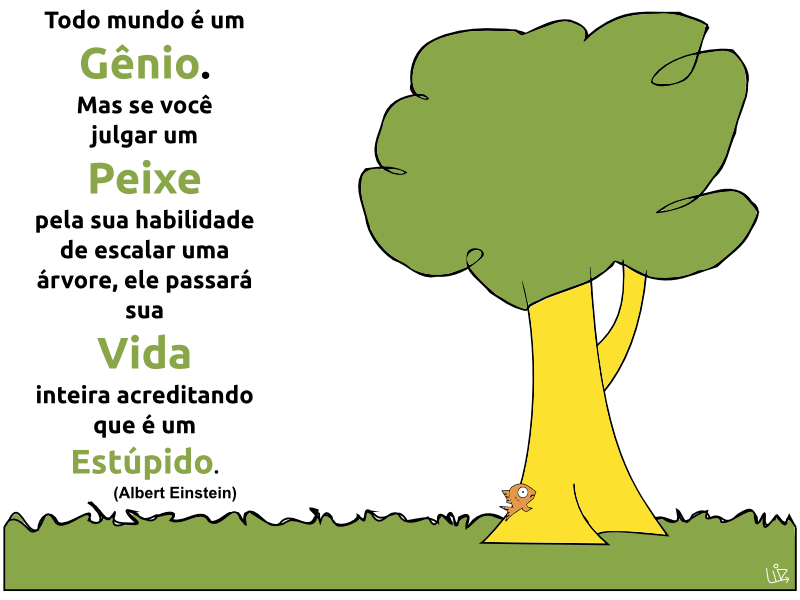
\includegraphics[scale=0.4]{figuras/todos-somos-genios}
 \caption{Exemplo de Figura.}
 \label{figurateste1}
\end{figure}

\begin{figure}[htb]
 \centering
  
\includegraphics[scale=0.8]{figuras/tux}
  \caption[Legenda mais curta.]{Esse é um exemplo de figura com legenda muito grande, que tem por objetivo mostrar como o espaço entre linhas será simples.}
  \label{figurateste2}
\end{figure}

\section{Segunda seção da Revisão.}

Em \eqref{equacao1} temos um exemplo de texto matemático com numeração\index{equação com numeração}. E logo depois 
temos um exemplo de texto matemático sem numeração.
%Note que o comando \index é usado para inserir "equação com numeração" no Índice.

\begin{equation}\label{equacao1}
 \int_a^b f'(x)\,dx = f(b) - f(a)
\end{equation}

\begin{equation}\nonumber
 \int_a^b f'(x)\,dx = f(b) - f(a)
\end{equation}

Aqui está mais outro exemplo de referência \cite{Autor4}.